\clearpage

\renewcommand{\ChapTitle}{Algorithms And Number Properties}
\renewcommand{\SectionTitle}{Algorithms And Number Properties}

\chapter{\ChapTitle}
\section{\SectionTitle}
\horizontalline{0}{0}

\subsection{Assigned Reading}

The reading assignments for this week can be found below:

\begin{itemize}
    \item \textbf{Sections 2.6, 3.1, 3.2, 4.2} from Rosen.
\end{itemize}

\subsection{Piazza}

Must post / respond to at least \textbf{two} Piazza posts this week. \due{(9/29/23)} \cbox{piazza-week5}

\subsection{Lectures}

The lectures for this week and their links can be found below:

\begin{itemize}
    \item \href{https://applied.cs.colorado.edu/mod/hvp/view.php?id=51632}{Algorithms} $\approx$ 36 min.
    \item \href{https://applied.cs.colorado.edu/mod/hvp/view.php?id=51633}{Complexity} $\approx$ 50 min.
    \item \href{https://applied.cs.colorado.edu/mod/hvp/view.php?id=51634}{Number Systems (Introduction) (F/S)} $\approx$ 13 min.
    \item \href{https://applied.cs.colorado.edu/mod/hvp/view.php?id=51635}{Conversion From Decimal To Binary (F/S)} $\approx$ 9 min.
    \item \href{https://applied.cs.colorado.edu/mod/hvp/view.php?id=51636}{Conversion Algorithm From Decimal To Binary (F/S)} $\approx$ 11 min.
    \item \href{https://applied.cs.colorado.edu/mod/hvp/view.php?id=51637}{Conversion Algorithm From Decimal To Any Base (F/s)} $\approx$ 9 min.
    \item \href{https://applied.cs.colorado.edu/mod/hvp/view.php?id=51638}{Binary / Hex To Decimal (F/S)} $\approx$ 11 min.
    \item \href{https://applied.cs.colorado.edu/mod/hvp/view.php?id=51639}{More Complexity And Matrix Multiplication} $\approx$ 44 min.
\end{itemize}

\noindent Below is a list of lecture notes for this week:

\begin{itemize}
    \item \pdflink{\LectureNotesDir Algorithms Lecture Notes.pdf}{Algorithms Lecture Notes}
    \item \pdflink{\LectureNotesDir Complexity Lecture Notes.pdf}{Complexity Lecture Notes}
    \item \pdflink{\LectureNotesDir Old School Sorting Lecture Notes.pdf}{Old School Sorting Lecture Notes}
\end{itemize}

\subsection{Assignments}

The assignment for this week is \pdflink{\AssDir Assignment 5 - Algorithms And Number Properties.pdf}{Assignment 5 - Algorithms And Number Properties} \due{(10/2/23)} \cbox{assignment-week5}

\subsection{Quiz}

The quiz's for this week can be found at \href{https://applied.cs.colorado.edu/mod/quiz/view.php?id=51641}{Algorithms And Numbers} \textbullet \pdflink{\QuizDir Quiz 5 - Algorithms And Matrices.pdf}{Quiz 5 - Algorithms And Matrices} \due{(10/2/23)} \cbox{quiz-week5}

\subsection{Chapter Summary}

The first section that we are covering this week is \textbf{Section 2.6 - Matrices}

\begin{notes}{Section 2.6 - Matrices}
    \subsubsection*{Overview}

    Matrices are fundamental mathematical structures used to represent and manipulate data in various fields, including mathematics, physics, computer science, engineering, and more. A matrix is 
    essentially a rectangular grid of numbers, symbols, or expressions arranged in rows and columns. It is a versatile tool for solving systems of linear equations, performing transformations, 
    and analyzing data. \vspace*{1em}
    
    Matrices have several key components and properties:
    
    \begin{enumerate}
        \item \textbf{Rows and Columns:} A matrix is defined by its dimensions, which specify the number of rows and columns it contains. For example, a matrix with three rows and two columns is 
        referred to as a "3x2 matrix."
    
        \item \textbf{Elements:} The entries within a matrix are called elements. These elements can be real numbers, complex numbers, or even variables and symbols.
    
        \item \textbf{Equality:} Two matrices are considered equal if they have the same dimensions and if their corresponding elements are equal. This forms the basis for matrix algebra.
    
        \item \textbf{Addition and Subtraction:} Matrices of the same dimensions can be added or subtracted by adding or subtracting their corresponding elements. This operation is done element-wise.
    
        \item \textbf{Scalar Multiplication:} A matrix can be multiplied by a scalar (a single number) by multiplying all of its elements by that scalar.
    
        \item \textbf{Matrix Multiplication:} Matrix multiplication is a more complex operation. It involves multiplying the rows of one matrix by the columns of another matrix and summing the 
        results. Notably, matrix multiplication is not commutative, meaning that the order of multiplication matters.
    
        \item \textbf{Identity Matrix:} The identity matrix is a special square matrix with ones on its main diagonal (from the top-left to the bottom-right) and zeros elsewhere. Multiplying any 
        matrix by the identity matrix leaves the matrix unchanged.
    
        \item \textbf{Transpose:} The transpose of a matrix is obtained by swapping its rows and columns. This operation is denoted by adding a superscript "T" to the matrix symbol.
    
        \item \textbf{Determinant:} The determinant of a square matrix is a scalar value that provides information about the matrix's invertibility and the scale factor of linear transformations 
        it represents.
    
        \item \textbf{Inverse:} Not all matrices have inverses, but square matrices that are invertible have an inverse matrix that, when multiplied by the original matrix, yields the identity matrix.
    \end{enumerate}
    
    Matrices are used in a wide range of applications, including solving systems of linear equations, representing geometric transformations, analyzing networks, performing data transformations, 
    and much more. They are a fundamental concept in linear algebra, and their versatility makes them a powerful tool for various mathematical and computational tasks.
\end{notes}

The next section that we are covering this week is \textbf{Section 3.1 - Algorithms}.

\begin{notes}{Section 3.1 - Algorithms}
    \subsubsection*{Overview}

    Algorithms are step-by-step procedures or sets of rules for solving specific problems or performing tasks. They are at the heart of computer science and play a pivotal role in various fields, 
    including mathematics, engineering, data science, and artificial intelligence. Algorithms are designed to take inputs, process them through a series of well-defined steps, and produce desired 
    outputs efficiently and accurately. \vspace*{1em}
    
    Key aspects of algorithms include:
    
    \begin{enumerate}
        \item \textbf{Problem Solving:} Algorithms are developed to address specific problems or tasks. They can range from simple tasks like sorting a list of numbers to complex challenges like 
        route optimization in logistics.
    
        \item \textbf{Efficiency:} Efficiency is a critical consideration in algorithm design. An efficient algorithm accomplishes its task with minimal resource usage, such as time and memory. 
        Efficient algorithms often have low time complexity, meaning they execute quickly, even for large inputs.
    
        \item \textbf{Correctness:} An algorithm must produce correct results for all valid inputs. Rigorous testing and mathematical proofs are used to ensure correctness.
    
        \item \textbf{Determinism:} Algorithms are deterministic, meaning that given the same input, they will produce the same output every time.
    
        \item \textbf{Termination:} An algorithm must eventually halt and produce an output. Infinite loops or non-terminating algorithms are considered faulty.
    
        \item \textbf{Analysis:} Analyzing an algorithm involves evaluating its performance, resource usage, and scalability. This analysis helps compare algorithms and select the most suitable 
        one for a given problem.
    
        \item \textbf{Data Structures:} Algorithms often work in conjunction with data structures, which are used to store and organize data efficiently. Common data structures include arrays, 
        linked lists, trees, and graphs.
    
        \item \textbf{Recursion:} Some algorithms use recursion, where a function calls itself to solve smaller instances of a problem. Recursion can simplify complex problems but requires 
        careful handling to avoid infinite recursion.
    
        \item \textbf{Complexity Theory:} Complexity theory categorizes algorithms based on their resource usage. It classifies algorithms as polynomial or exponential, helping understand their 
        computational limits.
    
        \item \textbf{Optimization:} Algorithms can be optimized to improve efficiency or reduce resource consumption. Optimization techniques may involve algorithmic improvements or parallel computing.
    
        \item \textbf{Applications:} Algorithms find applications in various domains, including computer graphics, cryptography, machine learning, data analysis, and network routing.
    
        \item \textbf{Algorithmic Paradigms:} Different algorithmic paradigms, such as divide and conquer, dynamic programming, and greedy algorithms, offer systematic approaches to problem-solving.
    
        \item \textbf{Algorithm Libraries:} Libraries and frameworks, like those in programming languages, provide pre-implemented algorithms, allowing developers to leverage well-tested solutions.
    
    \end{enumerate}
    
    Algorithms are the foundation of modern computing and enable the automation of tasks, from simple calculations to complex decision-making processes. Their study and development are central 
    to advancing technology and solving real-world challenges.    
\end{notes}

The next section that we are covering this week is \textbf{Section 3.2 - The Growth of Functions}.

\begin{notes}{Section 3.2 - The Growth of Functions}
    \subsubsection*{Overview}

    Algorithmic complexity refers to the analysis of how an algorithm's performance scales concerning the size of its input data. It provides insights into how efficiently an algorithm operates 
    and how its runtime or resource consumption grows as the input size increases. Big O notation is a mathematical notation used to express algorithmic complexity in a simplified and standardized 
    way. It allows us to categorize algorithms based on their upper bounds regarding time and space requirements.
    
    Key points about algorithmic complexity and Big O notation include:
    
    \begin{enumerate}
        \item \textbf{Time Complexity:} Time complexity measures the number of basic operations (such as comparisons or assignments) performed by an algorithm concerning the input size. It quantifies 
        how the runtime of an algorithm increases as the input grows. Algorithms are classified into categories like constant time ($O(1)$), linear time ($O(n)$), quadratic time ($O(n^2)$), and more 
        complex complexities ($O(n\log n)$, $O(2^n)$) based on their behavior.
    
        \item \textbf{Space Complexity:} Space complexity evaluates the memory usage of an algorithm in relation to the input size. It describes how additional memory requirements grow as the input 
        size increases. Similar to time complexity, algorithms can be categorized as using constant space ($O(1)$), linear space ($O(n)$), or more complex space complexities.
    
        \item \textbf{Big O Notation ($O$):} Big O notation provides an upper bound on the worst-case time or space complexity of an algorithm. It describes how an algorithm's performance scales 
        asymptotically (for very large inputs). For example, if an algorithm has a time complexity of $O(n^2)$, it means that its runtime will not grow faster than a quadratic function of the input 
        size.
    
        \item \textbf{Best, Average, and Worst Cases:} Algorithms may have different complexities depending on the input data's characteristics. The best-case complexity represents the most efficient 
        scenario, while the worst-case complexity describes the least efficient scenario. The average-case complexity provides an average estimate of performance over all possible inputs.
    
        \item \textbf{Comparing Algorithms:} Big O notation is invaluable for comparing and selecting algorithms for specific tasks. When faced with multiple algorithms to solve the same problem, 
        choosing the one with the lower Big O complexity often leads to better overall performance.
    
        \item \textbf{Trade-offs:} Optimizing one aspect of an algorithm's complexity may lead to trade-offs in other areas. For example, reducing time complexity may increase space complexity. 
        Analyzing these trade-offs is essential for algorithm design.
    
        \item \textbf{Practical Considerations:} While Big O notation is a useful tool, it simplifies the analysis. Practical considerations, like constant factors and hidden constants, may impact 
        real-world performance. Profiling and benchmarking are essential for fine-tuning algorithms.
    
        \item \textbf{Complexity Classes:} Complexity classes categorize problems based on their inherent computational difficulty. Classes like P (problems solvable in polynomial time) and NP 
        (non-deterministic polynomial time) are central to computer science and the theory of computation.
    
    \end{enumerate}
    
    Algorithmic complexity and Big O notation provide a structured approach to evaluating and comparing algorithms' efficiency and scalability. They are essential tools for computer scientists, 
    software engineers, and developers seeking to design and implement high-performance algorithms for a wide range of applications.

    \begin{highlight}[Runtime Examples]
        Below is an image that depicts examples of runtime operations in algorithms.

        \begin{center}
            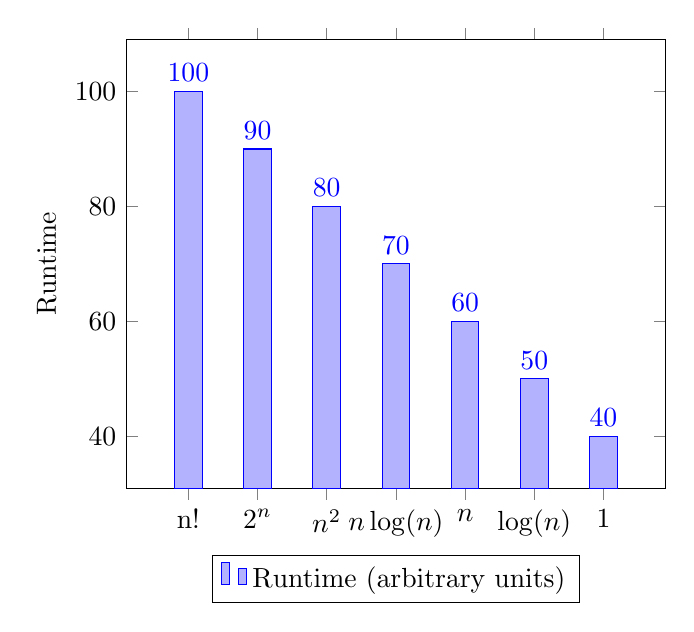
\begin{tikzpicture}
                \begin{axis}[
                    ybar,
                    enlargelimits=0.15,
                    legend style={at={(0.5,-0.15)},
                    anchor=north,legend columns=-1},
                    ylabel={Runtime},
                    symbolic x coords={n!, $2^n$, $n^2$, $n\log(n)$, $n$, $\log(n)$, $1$},
                    xtick=data,
                    nodes near coords,
                    nodes near coords align={vertical},
                    ]
                    \addplot coordinates {(n!,100) ($2^n$,90) ($n^2$,80) ($n\log(n)$,70) ($n$,60) ($\log(n)$,50) ($1$,40)};
                    \legend{Runtime (arbitrary units)}
                \end{axis}
            \end{tikzpicture}
        \end{center}

        The graph illustrates the runtime comparison of various functions with different algorithmic complexities. Each function is represented on the x-axis, including $n!$, $2^n$, $n^2$, $n \log(n)$, 
        $n$, $\log(n)$, and $1$. On the y-axis, the runtime is depicted in arbitrary units. The graph uses a ybar plot, and each bar corresponds to one of the functions, showing how their runtimes 
        compare. As expected, $n!$ (factorial) has the highest runtime, followed by $2^n$ and $n^2$. Conversely, constant-time complexity ($1$) has the lowest runtime, and other functions, like $n \log(n)$ 
        and $n$, fall in between. This graph provides a visual representation of how different algorithmic complexities impact runtime.

        Below is a table that summarizes commonly used terminology for the complexity of algorithms.

        \begin{center}
            \begin{tabular}[ht]{|c|c|}
                \hline \textbf{Complexity} & \textbf{Terminology} \\ \hline
                $\Theta(1)$ & \text{Constant Complexity} \\ \hline
                $\Theta(\log{(n)})$ & \text{Logarithmic Complexity} \\ \hline
                $\Theta(n)$ & \text{Linear Complexity} \\ \hline
                $\Theta(n \log{(n)})$ & \text{Linearithmic Complexity} \\ \hline
                $\Theta(n^{b})$ & \text{Polynomial Complexity} \\ \hline
                $\Theta(b^{n}),$ \text{ where $b > 1$} & \text{Exponential Complexity} \\ \hline
                $\Theta(n!)$ & \text{Factorial Complexity} \\ \hline
            \end{tabular}
        \end{center}
    \end{highlight}
\end{notes}

The last section that we will cover this week is \textbf{Section 4.2 - Integer Representation And Algorithms}

\begin{notes}{Section 4.2 - Integer Representation And Algorithms}
    \subsubsection*{Overview}

    In mathematics and computer science, various number bases are used to represent and work with numbers, each with its unique properties and applications. Here, we'll explore four common bases: decimal, 
    hexadecimal, octal, and binary.

    \begin{itemize}
        \item \textbf{Decimal (Base 10)} - Decimal is the base most commonly used by humans. It's a base-10 system, meaning it has ten digits: 0, 1, 2, 3, 4, 5, 6, 7, 8, and 9. In a decimal number, each 
        digit's position signifies a power of 10. For example, in the number 365, the digit 5 is in the one's place, 6 is in the ten's place, and 3 is in the hundred's place.

        \item \textbf{Hexadecimal (Base 16)} - Hexadecimal, often used in computing, is a base-16 system. It uses sixteen symbols: 0-9 for values 0 to 9 and A-F for values 10 to 15. Hexadecimal is compact 
        and frequently used to represent binary data in a more human-readable format. For example, the decimal number 255 is represented as FF in hexadecimal.

        \item \textbf{Octal (Base 8)} - Octal is a base-8 system, employing eight symbols: 0-7. It's less common today but was widely used in early computing. Octal numbers are sometimes used in Unix file 
        permissions, where each digit represents three bits of data.

        \item \textbf{Binary Base (Base 2)} - Binary is the fundamental base for computers, using only two symbols: 0 and 1. It's the language of digital circuits, where each bit represents an on/off state. 
        Computers store and manipulate data in binary form, making it critical in computer science.
    \end{itemize}

    Each of these bases serves specific purposes in different fields, with decimal being the most familiar to people in everyday life, while hexadecimal, octal, and binary are more commonly used in computer 
    science and digital technology. Understanding these bases is essential for working with various types of data and programming languages.
\end{notes}